\documentclass{article}
\usepackage[utf8]{inputenc}
\usepackage{graphicx}
\usepackage{fancyhdr}
\usepackage{amsmath}
\usepackage[dvipsnames]{xcolor}
\usepackage{amssymb}
\usepackage{amsthm}
\usepackage{dirtytalk}
\usepackage{array}
\usepackage{listings}
\usepackage{xcolor}

\definecolor{codegreen}{rgb}{0,0.6,0}
\definecolor{codegray}{rgb}{0.5,0.5,0.5}
\definecolor{codepurple}{rgb}{0.58,0,0.82}
\definecolor{backcolour}{rgb}{0.95,0.95,0.92}

\lstdefinestyle{mystyle}{
literate=
               {=}{$\leftarrow{}$}{1}
               {==}{$={}$}{1}
               {->}{$\rightarrow{}$}{1},
    backgroundcolor=\color{backcolour},   
    commentstyle=\color{codegreen},
    keywordstyle=\color{magenta},
    numberstyle=\Large \color{codegray},
    stringstyle=\color{codepurple},
    basicstyle=\ttfamily\footnotesize,
    breakatwhitespace=false,         
    breaklines=true,                 
    captionpos=b,                    
    keepspaces=true,                 
    numbers=left,                    
    numbersep=5pt,                  
    showspaces=false,                
    showstringspaces=false,
    showtabs=false,                  
    tabsize=2
}

\lstset{style=mystyle}

\theoremstyle{definition}
\newtheorem*{definition}{Definition}
\theoremstyle{example}
\newtheorem*{example}{Problem Statement}
\graphicspath{{./images/}}
\usepackage[a4paper, total={6in, 9in}]{geometry}


\title{\Huge \textbf{Data Structures and Algorithms}}
\author{\LARGE Akash Cherukuri - 190050009}
\date{\LARGE Computer Science and Engineering}

\setlength\parindent{24pt}

\pagestyle{fancy}
\fancyhf{}
\fancyhead[C]{\large \leftmark}
\fancyfoot[C]{\large \thepage}

\renewcommand{\headrulewidth}{1pt}
\renewcommand{\footrulewidth}{1pt}

\begin{document}

\maketitle

\begin{center}
    \LARGE
    \vspace{5mm}
    Mentor:- Prasanna Telawane
\end{center}

 \vspace{15mm}
 \hspace{-10mm}
    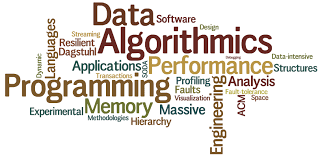
\includegraphics[scale = 1.5]{title.png}

\newpage
\Large
\tableofcontents
\newpage

\Large

\section{\Large Introduction}
\hspace{6mm} \textbf{Data Structures} are structures which are used to handle and store data. Data Structures may be present by default in a programming language, and if they aren't present in there, we can code them in. Having a good knowledge of data structures is essential as it allows the programmer to be able to manipulate the data as needed seamlessly and in an effortless manner.\par
\vspace{3.5mm}
An \textbf{algorithm} is a finite set of instructions or logic, written in order, to accomplish a certain predefined task. Algorithm is not the complete code or program, it is just the core logic(solution) of a problem, which can be expressed either as an informal high level description using a flowchart.

\subsection{\Large Prerequisites }
\subsubsection{\Large Debugging your Algorithm - Stress Testing}
\hspace{6mm}Creating and Coding of a better Algorithm than the existing one is challenging, and usually ends up having some mistakes in it. Usually, the programmer might forget some rare cases in which the algorithm fails, or worse, produces wrong results. It can also be seen that debugging of such a case is difficult, as the problem doesn't occur frequently. \textbf{Stress-Testing} can be employed to identify some of these bugs. \par
\vspace{5mm}
Stress-Testing is an exhaustive method of testing your bugs, in which the inputs are generated randomly. It is carried out by repeatedly giving the same inputs to both the algorithms (the older one and the faster, more efficient newer one) and checking whether the output produced by both the algorithms is the same or not. By the use of \textbf{cout} (in C) or \textbf{print} (in Python) statements, we can identify the cases in which our algorithm(s) fail, and debug them appropriately. \par
\newpage
\noindent \textbf{An Example of Stress Testing is shown Below:-}\par
\vspace{5mm}

\noindent \hspace{2mm} \texttt{\textcolor{gray}{//f1 is the first algorithm, f2 is the second algorithm.}}\par
\noindent \hspace{2mm} 
\texttt{\textcolor{violet}{while}(\textcolor{orange}{TRUE})\{ }\par
\noindent \hspace{12mm}
\texttt{x\textcolor{cyan}{=}\textcolor{NavyBlue}{rand}()\%\textcolor{orange}{100};}\par
\noindent \hspace{12mm}
\texttt{cout \textcolor{cyan}{<<} \textcolor{LimeGreen}{"Input:"} \textcolor{cyan}{<<} x \textcolor{cyan}{<<} endl;}\par
\noindent \hspace{12mm}
\texttt{res1 \textcolor{cyan}{=} f1(x);}\par
\noindent \hspace{12mm} \texttt{res2 \textcolor{cyan}{=} f2(x);} \par
\noindent \hspace{12mm} \texttt{\textcolor{violet}{if}(res1\textcolor{cyan}{!=}res2)\{} \par
\noindent \hspace{22mm} \texttt{cout \textcolor{cyan}{<<} \textcolor{LimeGreen}{"Error"} \textcolor{cyan}{<<} endl;}\par
\noindent \hspace{22mm} \texttt{cout \textcolor{cyan}{<<} res1 \textcolor{cyan}{<<} \textcolor{LimeGreen}{" "} \textcolor{cyan}{<<} res2 \textcolor{cyan}{<<} endl;} \par
\noindent \hspace{22mm} \texttt{\textcolor{violet}{break};} \par
\noindent \hspace{12mm} \texttt{\}}\par
\noindent \hspace{12mm} \texttt{\textcolor{violet}{else} cout \textcolor{cyan}{<<} \textcolor{LimeGreen}{"OK"} \textcolor{cyan}{<<} endl;}\par
\noindent \hspace{2mm}\texttt{\}}

\subsubsection{\Large Pseudo-Code}
\hspace{4mm}Because data structures and Algorithms are universally applicable to all languages, it doesn't make sense to talk about the logic in terms of a single programming language. Neither can we just simply state the logic as it may not be understood by everyone. \par 
\vspace{4mm}
Therefore, in order to express the logic, we use an informal high-level description of the logic. Further more, we can make it so that our descriptions follow the general coding syntax, without actually using a programming language.\par
\vspace{4mm}
This informal descrition of the logic in an alforithm is reffered to as \textbf{Pseudo-Code}. Pseudo-Code means "False Code", and it is called so because the description \textit{looks} like a code, but is not.


\section{\Large Algorithms}
\hspace{6mm} As previously discussed, and Algorithm is just a set of instructions which can be followed to solve a specific set of problems. Being able to create, and code, efficient algorithms is a very important skill that every programmer must try to include in his/her skillset. \par
\subsection{\Large What makes an Algorithm good?}
\hspace{6mm} An Algorithm is said to be \textbf{"good"} or \textbf{"better"} than a different algorithm when both the algorithms are designed to perform the same tasks, but the first algorithm excels the second Algorithm in any of the following criteria :-
\begin{itemize}
    \item It takes lesser time to arrive at the solution.
    \item It is computationally less heavy.
    \item It uses up lesser computational resources.
\end{itemize}
\vspace{5mm}
\noindent \LARGE \textbf{Example of a good Algorithm} \par
\Large
\vspace{3mm}Suppose we would like to create a program to compute the value of the $n^{th}$ number in the Fibonacci Series. A trivial way of coding this in would be to have and iterated function as follows: \par

\vspace{5mm}
\noindent \hspace{10mm} \texttt{\textcolor{gray}{//Recursive version of the code}}\par
\noindent \hspace{10mm} \texttt{\textcolor{violet}{int} Fib\_Calc(\textcolor{violet}{int} n)\{} \par
\noindent \hspace{20mm} \texttt{\textcolor{violet}{if}(n\textcolor{cyan}{<=}\textcolor{orange}{1}) \textcolor{violet}{return} n;}\par
\noindent \hspace{20mm} \texttt{\textcolor{violet}{else return} (Fib\_Calc(n\textcolor{orange}{-1})\textcolor{cyan}{+}Fib\_Calc(n\textcolor{orange}{-2}));}\par
\noindent \hspace{10mm} \texttt{\}}
\vspace{5mm}

 This Algorithm for calculating the $n^{th}$ number seems to be very simple and straight-forward, but is highly inefficient. For example, if we needed the $100^{th}$ number in the series, the program running on this code wouldn't be able to calculate it simple because of how inefficient this method is.
To understand why this inefficient, lets try to create a Binary Tree model for the way in which the $n^{th}$ number in the sequence, say $F_n$ is calculated: \newline

 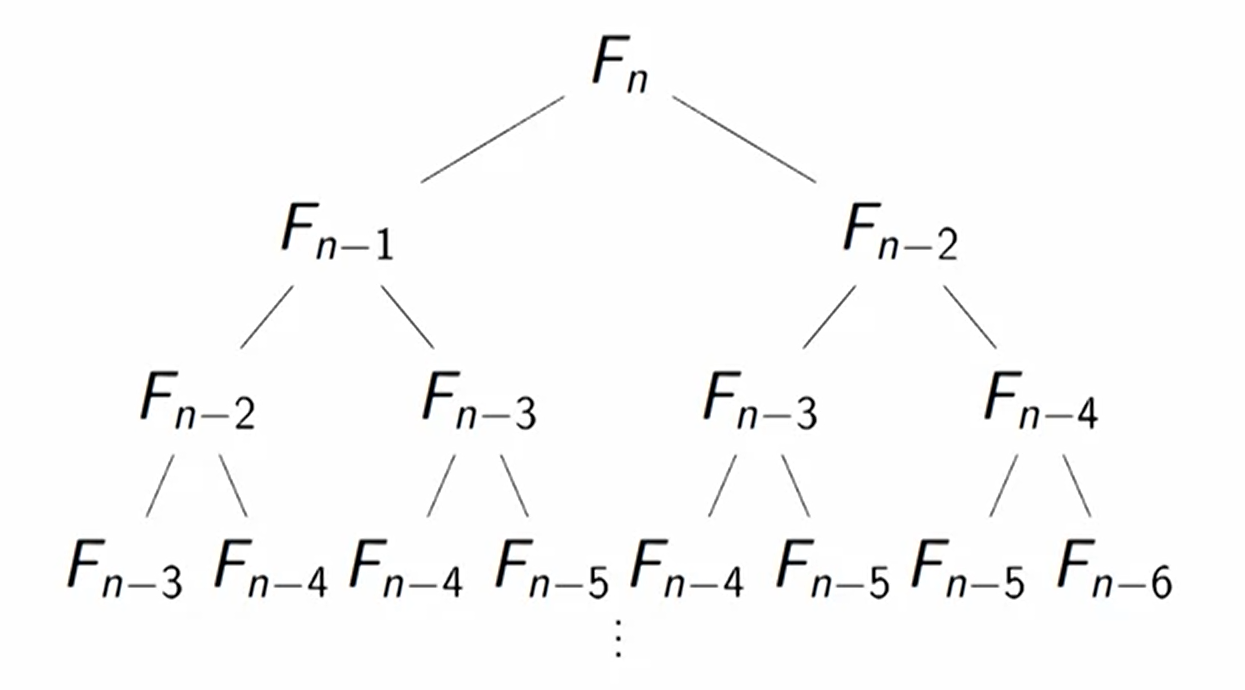
\includegraphics[scale = 0.5]{Bin.png}\par

 Notice how $F_{n-3}$ is being calculated thrice unnecessarily? This is what causes our algorithm to be very tedious computational-wise and what causes it to be very time consuming. In order to overcome this, we could devise another algorithm which actually stores the values of Fn as it goes upto the required value of $n$ as follows:\par

\vspace{5mm}
\noindent \hspace{30mm} \texttt{\textcolor{gray}{//New Algorithm for the task}}\par
\noindent \hspace{30mm} \texttt{\textcolor{violet}{int} Fib\_Calc(\textcolor{violet}{int} n)\{}\par
\noindent \hspace{40mm} \texttt{\textcolor{violet}{int} i\textcolor{cyan}{=}\textcolor{orange}{2};}\par
\noindent \hspace{40mm} \texttt{\textcolor{violet}{int} val[n\textcolor{orange}{+1}];}\par
\noindent \hspace{40mm} \texttt{val[\textcolor{orange}{0}] \textcolor{cyan}{=} \textcolor{orange}{0};}\par
\noindent \hspace{40mm} \texttt{\textcolor{violet}{while}(\textcolor{orange}{TRUE})\{}\par
\noindent \hspace{50mm} \texttt{val[i] \textcolor{cyan}{=} val[i\textcolor{orange}{-1}]\textcolor{cyan}{+}val[i\textcolor{orange}{-2}];}\par
\noindent \hspace{50mm} \texttt{\textcolor{violet}{if}(i\textcolor{cyan}{==}) \textcolor{violet}{return} val[n];}\par
\noindent \hspace{50mm} \texttt{i\textcolor{cyan}{++};}\par
\noindent \hspace{40mm} \texttt{\};}\par
\noindent \hspace{30mm} \texttt{\}}\par

This is a better algorithm when compared with our previously written recursive algorithm, as it calculates the values \textbf{QUICKER} then the first algorithm, and it also is \textbf{COMPUTATIONALLY LESS HEAVY}.\par
\vspace{5mm}
From this example, we can see understand the importance of studying and understanding and the power of being able to write good Algorithms. A good algorithm is what makes the difference between a solution being given out in a million years, or a solution being given out as soon as we hit run. It is what makes the searching through trillions of webpages be done within seconds, and it is what is the most versatile, and arguable, on of the most important topics to be understood properly.

\subsection{\Large Computing Runtimes}
\hspace{6mm}We've been talking about an algorithm being faster than another and about an algorithm being more efficient than the other. So, the next logical question to be posed would be, "How long in general would the algorithm take to finish a computation?" This question opens up a whole new can of worms, as it cannot be answered very easily.\par
\vspace{5mm}
We can see why this would be a difficult question to answer as there are many factors which can cause the runtime of an algorithm to vary, like the difference in the computational power of different clients and the different number of computations to be performed when the inputs are different, to name a few. One might think of a workaround to count the number of lines of code being run.\par
\vspace{5mm}

However, this would be very vague as different lines of code would require different degrees of computational power. For example, a line involving addition of two numbers and another initialising an array of numbers would obviously different time.\par
\vspace{2mm}
\begin{center}
    \textbf{IDEA: Assume that all the above issues affect the runtime by a constant factors, which we can ignore.}
\end{center}
\vspace{2mm}
\hspace{6mm}That is, a client who has a slow computer might cause the speed of computation of ALL processes to be doubled. This idea, however, is a little problematic as then runtimes of a second and an year would be considered the same as they differ by a constant multiple. This problem is solved by talking about runtimes in an \textbf{Asymptomatic Notation}.

\subsubsection{\Large Asymptomatic Notation}

\hspace{6mm}Asymptomatic Notation or Asymptomatic Method of talking of runtimes invloves thinking about how the runtimes scale with respect to the size of the input data. This makes sense, as when the input data is Large enough, an algorithm whose runtime scales as $n^2$ would be significantly worse than one which scales as $1000n$.\par
\vspace{5mm}
The maximum time that an algorithm must take can be defined by us, and from that we can calculate a good estimate of the maximum input size that the algorithm can compute, given that we know the \textbf{scaling} of the algorithm. \textbf{"Scaling"} refers to how the runtime depends on the input size.\par
\vspace{3mm}
\begin{center}
    \textbf{General Scaling Comparisions}
\end{center}
\[log_a n < \sqrt[n]{x} < n < n log_a n < n^a < a^n \]
\[a \in \mathbb{N} \]
\newpage
\subsubsection{\Large Big-O Notation}
\hspace{6mm}Big-O is a notation which takes the ideology of Asymptomatic Notation and gives it a mathematical definition. This notation allows us to be able to quantitatively descern \textit{How Fast} our algorithm is.\par
\vspace{4mm}

\theoremstyle{definition}
\begin{definition}{}
    Let $f$ and $g$ be two functions. "$f$ is Big-O of $g$", or, $f(n) = O(g(n))$ when $\exists$ $N, c \in \mathbb{Q}^+$ such that $f(n) \leq c\cdot g(n)$ $\forall$ $n\geq N$.
\end{definition}
\vspace{4mm}

We can see from the above definition that the Big-O notation tells us about the \textbf{Upper Bound} for the number of operations that would need to to be performed by the computer when following the algorithm. This notion has many advantages, some of them being:

\begin{itemize}
    \item Clarifies growth rates for large sized inputs
    \item Clean notations for better representation and understanding
    \item Mathematically quantified $\implies$ Algebra is possible
    \item For large enough inputs, choosing a faster algorithm is easy.
\end{itemize}

\noindent \textbf{Algebra of Big-O notation}
\begin{enumerate}
    \item Multiplicative Constants can be ignored \newline
            $7n^2 = O(n^2)$
    \item Smaller terms can be ignored \newline
            $n^2 + 3n + log_a^n = O(n^2)$
    \item $a,b \in \mathbb{Q}^+$, $a < b$ $\implies$ $n^a = O(n^b)$
    \item $a,b \in \mathbb{Q}^+$ and $a > 0, b > 1$ $\implies$ $n^a = O(b^n)$
    \item $a,b \in \mathbb{Q}^+$ $\implies$ $(logn)^a = O(n^b)$
\end{enumerate}

By using the above algebra and our intuition, we can accurately talk about the upper bound of the runtime of the algorithm. Consecutive steps in the algorithm require us to add the Big-O functions, while those in a loop require us to multiply the Bog-O function of the steps \textbf{IN} the loop with the Big-O function of the looping mechanism itself. We then further simplify the Big-O notation and arrive at our Final Answer.\par
\vspace{5mm}
However, this noation of representing runtimes is not without faults. The faults of this notation are given below:
\begin{itemize}
    \item Runtimes which differ by a constant factor cannot be distinguished by this notation.
    \item By definition, Big-O is asymptomatic in nature.
    \item It works well only for Large sizes of data. An Algorithm which follows $n^3$ (for example) is faster than $3^n$ for small sizes of data. 
\end{itemize}

\subsubsection{\Large $\Omega$-Notation and $\Theta$-Notation}

\hspace{6mm}$\Omega$-Notation is just like the Big-O notation, but it tells us about the lower bounds of the runtime.

\theoremstyle{definition}
\begin{definition}{}
    Let $f$ and $g$ be two functions. "$f$ is $\Omega$ of $g$", written as, $f(n) = \Omega(g(n))$ when $\exists$ $N, c \in \mathbb{Q}^+$ such that $f(n) \geq c\cdot g(n)$ $\forall$ $n\geq N$.
\end{definition}
\vspace{4mm}
All the algebra of Big-O is still valid for $\Omega$ with logic reversed. That is, instead of the smaller terms being ignored, we ignore the larger terms and the such.\par
\vspace{5mm}
$\Theta$-Notation is similar to an equality in Algebra. It tells us that the functions increase at a similar rate.
\theoremstyle{definition}
\begin{definition}{}
    Let $f$ and $g$ be two functions. "$f$ is $\Theta$ of $g$", written as, $f(n) = \Theta(g(n))$ iff $f(n) = O(g(n))$ and $f(n) = \Omega(g(n))$
\end{definition}
For example, $3n^2+5n+3 = \Theta(n^2)$

\subsubsection{\Large Master Theorem}
\hspace{4mm} This theorem is used to quickly find the run-times of an algorithm in terms of the Big-O notation, when the relations are in recursive format, \(T(n) = aT(\frac{n}{b}) + O(n^d)\). The formula is as follows:
\[   T(n)\left\{
\begin{array}{ll}
      O(n^d) & d > log_b^a \\
      O(n^dlogn) & d = log_b^a \\
      O(log_b^a) & d < log_b^a \\
\end{array} 
\right. \]

\subsection{\Large Types of Algorithms}
\hspace{5mm} An algorithm in development has different stages to it, and its development cycle mostly goes along the steps:

\begin{enumerate}
    \item \textbf{Naive Algorithm:} This algorithm is derived from the definition of the problem statement. It's usually slow and requires optimization.
    \item \textbf{Optimized Algorithm:} The naive algorithm is optimized by using some standard tools(discussed below) or by the usage of data structures and reorganizing the way in which steps are done in the algorithm.
    \item \textbf{"Magic" Algorithm:} This is completely different from the above two, in the sense that it uses a unique insight into the problem, and requires a good understanding of the problem statement.
\end{enumerate}

There are different ways of optimizing the Naive Algorithm, which are given below. However keep in mind that there is no Silver Bullet for this problem, as no method, that we know of, will work for all the infinitely many types of problem statements. With that being said, it is up to the programmer to decide which method would work, and this requires them to have a good grasp of the methods.

\subsubsection{\Large Greedy Algorithms}
\hspace{6mm}These classes of algorithms work out an optimised solution for a given problem statement by taking the most "greedy" step at a localised level, and then they repeat this till they reach the end. For example, a shortest path finding algorithm working in this way would choose the option which takes it closest to the destination, and then it repeats this till it reaches the solution.\par
\vspace{4mm}
Before we move further, we must define some terms so that it is easier to understand some core concepts of this class of Algorithms.\par\newpage
\vspace{5mm}
\noindent \textbf{Sub Problem:}\par
\vspace{2mm}
A Sub-Problem is a problem which belongs to the same problem-class as the original problem statement, and is smaller than the original problem statement.\par
\vspace{3mm} In the previous path-finding example problem, finding a path from the end of the greedy step to the end would constitute as a sub problem.\par
\vspace{5mm}
\noindent \textbf{Safe Step:}\par
\vspace{2mm}
An option among the many present at any given point is considered to be "Safe", if there exists an optimized path from the end of this step to the end of the original problem.\par
\vspace{4mm}
A safe step may, or may not be intuitive in nature as that depends on the complexity of the problem statement. Therefore, it generally is a good practice to prove mathematically that the steps being taken by your algorithm are all safe. \par
\vspace{4mm}
\noindent Now that the definitions of a safe step and a Sub-Problem are clear, lets look at how a Greedy Algorithm can be coded to work:

\begin{enumerate}
    \item \textbf{Reduce the given problem statement to a mathematical model.} This makes the following steps easier, and proving that the steps taken are safe into a mathematical problem, instead of one relying on intuition.
    \item \textbf{Determine the Greedy Step.} This is a step which takes the algorithm closest to the end point of the problem, where the computation becomes so easy that it can be computed manually.
    \item \textbf{Prove that the Greedy Step taken is Safe.}This ensures that there are no exceptions left out. This is critical, because if we finish coding an algorithm whose greedy steps aren't safe, we would need to scrap the entire thing.
    \item \textbf{Ensure that once the Greedy Step is taken, the problem becomes a Sub-Problem.} If it doesn't either the logic of our greedy step is wrong or the algorithm can't be coded in this fashion.
\end{enumerate}

\subsubsection{\Large Divide and Conquer Algorithms}
\hspace{5mm}As the name suggests, this class of Algorithms aims to solve a problem by dividing it into smaller \textbf{Sub-Problems}, solving each one of them, and then using the answers from all the sub parts to produce the final answer. Although it looks very similar to the Greedy Algorithm, ONE key difference they both have is:
\begin{itemize}
    \item In Divide and Conquer algorithms, division occurs first and then the computation follows.
    \item In Greedy Algorithms; computation occurs, then forming a sub-problem follows automatically, and then this loop is repeated till we reach our destination. 
\end{itemize}
Example of some problem-statements where this methodolgy is used would be:-
\begin{itemize}
    \item Binary Search
    \item Polynomial Multiplication
    \item Sorting Algorithms
\end{itemize}
We shall look at Polynomial Multiplication in detail now.\par
\subsubsection*{\Large Polynomial Multiplication}
The problem statement is straightforward; Given two polynomials of degrees $n$ and $m$, what is their product?\par
\vspace{4mm}
\noindent \textbf{Naive Algorithm}\par
\vspace{2mm}
Let us first define that the input of our problem to be $n$ (the max degree between the two polynomials), followed by the co-efficients of the polynomials from $x^{n}$.\par
\vspace{4mm}
Let the polynomials be: \[A(x) = a_{n-1}x^{n-1} + a_{n-2}x^{n-2} + ... + a_1x + a_o\]\[B(x) = b_{n-1}x^{n-1} + a_{n-2}x^{n-2} + ... + b_1x + b_o\]
And let the product of these two polynomials be: \[P(x) = p_{2n-2}x^{2n-2} + p_{2n-3}x^{2n-3} + ... + p_1x + p_o\]
We can quite easily calculate the value of each $p_i$ by the following formula:
\[p_i = \sum_{j=0}^{i} a_jb_{i-j}\]
A naive Algorithm can be set up from the formula. But let's look at the time it would take this algorithm to actually compute the product. For every $p_i$, we would need to perform addition at least $n$ times; and this would need to be repeated for $2n$ tries to calculate all the co-efficients.\par
\vspace{4mm}
Therefore, the run-time of out naive algorithm is \textbf{\(O(n^2)\)}.\par
\vspace{4mm}
\noindent \textbf{Divide and Conquer Algorithm} \par
\vspace{4mm}
To reduce the run-time, let's try to implement a divide and conquer strategy. Let's split the given polynomials $A(x)$ and $B(x)$ as follows:
\[A(x) = C(x)\cdot x^{n/2} + D(x)\] \[B(x) = E(x)\cdot x^{n/2} + F(x)\]
(if n is not even, just pad the polynomial by adding zero terms)
\[A(x)\cdot B(x) = \{C(x)\cdot E(x)\}x^n + \{C(x)\cdot F(x) + D(x)\cdot E(x)\}x^{n/2} + D(x)\cdot F(x)\]
Notice how we've broken the problem down in \textbf{FOUR} sub problems, half as big as the original. The four sub-Problems are the product of the polynomials in the RHS of the above equation. Keep in mind that the degree of each of the sub-problem is $(n/2)-1$\par
\newpage
\noindent Let's look at the Pseudo-Code for this Algorithm:\par
\vspace{3mm}
\noindent \texttt{\textcolor{violet}{Function} Multiply(A, B, n, ai, bi):} \par
\noindent \hspace{10mm} \texttt{res = \textcolor{orange}{array}[2n-1];}\par
\noindent \hspace{10mm} \texttt{\textcolor{violet}{if} n\textcolor{cyan}{==}\textcolor{orange}{1} :} \par
\noindent \hspace{20mm} \texttt{res[\textcolor{orange}{0}] = A[i] * B[j];} \par
\noindent \hspace{20mm} \texttt{\textcolor{violet}{return} res;} \par
\noindent \hspace{10mm} \texttt{\textcolor{gray}{//Calculating D(x)*F(x)}}\par
\noindent \hspace{10mm} \texttt{res[0, ... n-2] = \textcolor{violet}{Multiply}(A, B, n/2, ai, bi);}\par
\noindent \hspace{10mm} \texttt{\textcolor{gray}{//Calculating C(x)*E(x)}}\par
\noindent \hspace{10mm} \texttt{res[n, ... 2n-2] = \textcolor{violet}{Multiply}(A, B, n/2, ai+n/2, bi+n/2);}\par
\noindent \hspace{10mm} \texttt{\textcolor{gray}{//Adding the value of middle term}}\par
\noindent \hspace{10mm} \texttt{CF = \textcolor{violet}{Multiply}(A, B, n/2, ai+n/2, bi);}\par
\noindent \hspace{10mm} \texttt{DE = \textcolor{violet}{Multiply}(A, B, n/2, ai, bi+n/2);}\par
\noindent \hspace{10mm} \texttt{res[(3n/2)-2 ... , n/2] += CF + DE;}\par
\noindent \hspace{10mm} \texttt{\textcolor{violet}{return} res;}
\vspace{4mm}

Let's carry out an analysis for the time taken. Assuming that n is a power of 2, (even if it isn't we can the pad the polynomials), the number of sub-problems that we will have at depth of division $i$ is equal to $4^i$, because each division further divides each product into four smaller products.\par
\vspace{4mm}
The work done for size $n$ in this algorithm is $kn$, because the calculated values of the co-efficients need to be assigned to the the array res, as seen in the above pseudo-code.\par
\vspace{4mm}
Therefore, work done at a given depth $i$ is given by: \[4^i\cdot k(\frac{n}{2^i}) = k\cdot 2^in\] 
But the value of $i$ is $log_2^n$, and this would mean work done at last step is \(k\cdot n^2\). So this would mean that this algorithm is also not better than the naive algorithm. However, as we shall see next, there is scope for improving this algorithm.\par
\vspace{4mm}
\newpage
\noindent \textbf{Optimized Divide and Conquer Algorithm or Karatsuba's Approach} \par
\vspace{4mm}
The reason why our algorithm is still slow is because 4 sub-problems are created in each step. This approach aims to reduce the number of sub-problems created by some clever mathematics.\par
\vspace{4mm}
The second term in the above algorithm's method is  $C(x)\cdot F(x) + D(x)\cdot E(x)$. However, we can write it more efficiently as: \[C(x)\cdot F(x) + D(x)\cdot E(x) = [C(x) + D(x)]\cdot [E(x) + F(x)] - C(x)\cdot E(x) - D(x)\cdot F(x)\]
This might seem cumbersome, but notice that the problem is divided into only 3 new sub-problems, namely, $[C(x) + D(x)]\cdot [E(x) + F(x)]$, $C(x)\cdot E(x)$ and $D(x)\cdot F(x)$. This is a game changer, as the work to be done now becomes $3^{log_2^n}$ or approximately $n^{1.58}$. We can truly appreciate how much better this is for very large values of $n$.

\subsubsection{\Large Dynamic Programming}
\hspace{4mm} This is yet another method of solving problems and optimizing naive algorithms. This is not a class of Algorithms per se, but rather is a clever application of logic and the constraints which are presented by the problem statement. \par
\vspace{4mm}
As Dynamic Programming is not a concept, but rather an idea, we can understand it via the following example:\par
\vspace{4mm}
\theoremstyle{example}
\begin{example}
    You are a cashier, and as part of your job is returning change. You would like to know the least number of coins needed for the transaction.
\end{example}
One of the first ideas that we would have to solve this problem would we to use a Greedy Algorithm. Like, find the largest coin which is smaller than the change. Use it, and repeat. This intuition isn't wrong, and it does in fact yield correct answers as shown:\newpage

\begin{itemize}
    \item Values of coins that we have: 1, 5, 10, 25
    \item Change to be returned: 42
    \item Using Greedy Algorithm, we get that the coins are 25, 10, 5, 1, 1.
\end{itemize}
However, It doesn't work for all cases as we can see below:

\begin{itemize}
    \item Values of coins that we have: 1, 5, 10, 20, 25
    \item Change to be returned: 40
    \item Using Greedy Algorithm, we get that the coins are 25, 10, 5.
\end{itemize}
However, notice that using two 20 coins is more efficient! Greedy Algorithm doesn't work because we haven't proved that using the highest possible denomination is a Safe Move.\par
\vspace{3mm} \noindent

\noindent \textbf{Solving this problem using Dynamic Programming} \par
\noindent Let us first define the terms Mathematically;
\begin{itemize}
    \item Optimal number of coins for Change $m$ is given by $C(m)$
    \item There are $n$ coins.
    \item Value of $i^{th}$ coin is given by $v_i$
    \item The coins are sorted in increasing order of value
\end{itemize}
\noindent By observing the problem statement, we can easily develop this recursive statement:
\[C(m) = min\{C(m-v_i) + 1, C(m-1)\} \forall v_i \leq m\]
\hspace{4mm}That is, the optimal solution can be obtained by backtracking. This is why this works: Suppose that the optimal number of coins to return a change of $x$ is $n$. Obviously, the optimal number of coins to return a change of $x+v_i$ is $n+1$! The above relation is just this logic in reverse.\par
\vspace{4mm}
So the idea that we might get would be to write a recursive algorithm which branches out from $C(m)$; which can be shown by the following Pseudo-Code:\newpage

\noindent \texttt{\textcolor{gray}{//Pseudo-Code for number of Coins}} \par
\noindent \texttt{\textcolor{violet}{Function} Coins(m):} \par
\noindent \hspace{10mm} \texttt{\textcolor{violet}{for} $v_i$ \textcolor{cyan}{$\leq$} m:} \par
\noindent \hspace{20mm} \texttt{rec = \textcolor{orange}{min}(Coins($m-v_i$) + 1, Coins($m-1$));} \par
\noindent \hspace{10mm} \texttt{\textcolor{violet}{return} rec;}\par
\vspace{4mm}
However, notice that a certain value of Coins(x) will be calculated many times over. Re-calculating this value many times will slow down the algorithm. Also, recall that this situation is highly similar to the Fibonacci Numbers problem that we had encountered earlier.\par
\vspace{4mm}
So we can use the same solution that we had used for the Fibonacci Series here as well. That is, in order to prevent recalculations, we create an array which stores the values of the optimal number of coins for a given number of change, and then values can be pulled directly from this array to save computation time.\par
\vspace{5mm}
\noindent\textbf{The Pseudo-Code for this idea is:}\par
\vspace{3mm}
\noindent\texttt{\textcolor{gray}{//Pseudo-Code for Better Algorithm}}\par
\noindent\texttt{\textcolor{violet}{Function} Fast\_Coins(m):} \par
\noindent\hspace{10mm} \texttt{val = \textcolor{violet}{arr}[m+1]; i=1;}\par
\noindent \hspace{10mm} \texttt{val[0] = 0;} \par
\noindent\hspace{10mm} \texttt{while i!=m:}\par
\noindent \hspace{20mm} \texttt{\textcolor{violet}{for} $v_i$ \textcolor{cyan}{$\leq$} i:} \par
\noindent \hspace{30mm} \texttt{rec = \textcolor{orange}{min}(val[$i-v_i$] + 1, val[$i-1$]);} \par
\noindent \hspace{30mm} \texttt{i++;}\par
\noindent \hspace{10mm} \texttt{\textcolor{violet}{return} val[m-1];} \par
\vspace{5mm}
This is the philosophy of Dynamic Programming. Instead of calculating the values over and over again in a recursion; we store the required values and look them up whenever needed.\par
\vspace{4mm}
However, this might rise a funny question in our heads, "Why is this called \textit{Dynamic Programming} in the first place?" The answer has a historic significance regarding its inception into Computer Science. The concept of Dynamic Programming was introduced by Richard Bellman in the 1950s while he was working on an Air Force Project.\par
\vspace{4mm}
However, when he introduced this, everyone dismissed this idea as it seemed non-sensical. We can see why they thought so as well, as it seems illogical to compute all the values till the required answer. However, we know mathematically that this wasn't the case! Richard wanted to hide the fact that he was really doing mathematics from the Secretary of Defense. The following quote from him drives the fact home:\par
\vspace{4mm}
\say{..what name do I chose? I was interested in planning, but planning is not a good word for various reasons. I decided to therefore use the word \say{programming} and I wanted to get across the idea that this was dynamic..}

\section{\Large Data Structures}
\hspace{4mm}As we've discussed earlier, Data Structures are structures which are used to handle and store data. Data Structures may be present by default in a programming language, and if they aren't present in there, we can code them in. Having a good knowledge of data structures is essential as it allows the programmer to be able to manipulate the data as needed seamlessly and in an effortless manner. \par

\subsection{\Large Arrays}
\begin{itemize}
    \item Arrays are a type of Data Structures in which data is stored in partitions of \textbf{Equal Size}.
    \item The partitions must have \textbf{continuous indexing}. The starting index can be 0, 1, or it can be defined by the user.
    \item It has \textbf{Constant Time access}, meaning that the time taken for accessing the array elements takes $O(1)$ time.
\end{itemize}
Also, the address of any element in the array can be deduced from the address of the array as follows:
\[Elem\_Addr = Array\_Addr + (Size of Partitions)\cdot (i - index\_of\_first)\]\par
\vspace{8mm}
Arrays also have the functionality to be \textbf{Multi-Dimensional}. There are two ways in which this may be done:
\begin{itemize}
    \item \textbf{Row-Major: }The elements are filled in Row-after-row, and we go to the next column after the row has been filled.
    \item \textbf{Column-Major: }The elements are filled in Column-wise, and we move to the next row once all the columns have been filled.
\end{itemize}

\subsection{\Large Singly-Linked List}
\hspace{4mm} A singly linked list is generally defined by the programmer, and it can be easily done recursively. A singly-linked list has \textbf{head pointer}, which points to a \textbf{node}. A node consists of variables to store data and a pointer which either points to the next node or points to None, if it is the end.\par
\vspace{2mm}
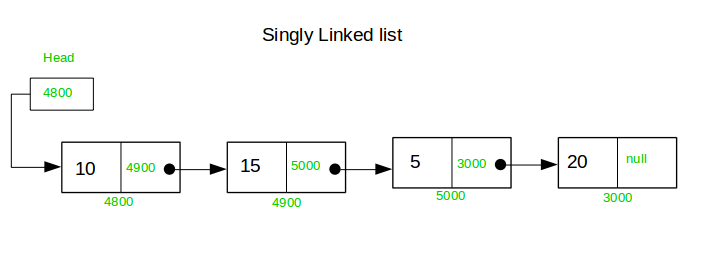
\includegraphics[scale = 0.75]{sll.png}\par
\vspace{2mm}
A variation of the singly-linked list has a \textbf{Tail Pointer}, which points to the last node in the entire structure. The advantage of having a tail-pointer is to quickly get to the element at the end of the linked list. Also keep in mind that moving from one element to another is possible \textbf{ONLY} in the forward direction.\par
\newpage
\subsubsection*{\Large Available functions and their run-times:}
\vspace{-2mm}
\begin{center}
 \begin{tabular}{| m{9em} | m{15em} | m{4.5em} |} 
 \hline
 \textbf{Function} & \textbf{Functionality} & \textbf{Runtime}\\ [0.5ex] 
 \hline
 pushfront(node) & Adds the node to the front & $O(1)$ \\ 
 \hline
 top() & Returns the top node & $O(1)$ \\
 \hline
 pop($i$) & Removes the $i^{th}$ node & $O(n)$ \\
 \hline
 append(node) & Adds the given node to end & $O(n)$ \\
 \hline
 find(node) & Searches for the given key, returns True if found & $O(n)$ \\ [1ex] 
 \hline
 add(node, key) & Adds the node after the given key & $O(n)$ \\
 \hline
\end{tabular}
\end{center}
\vspace{3mm}
Notice that the runtime for the $append(node)$ function can be reduced from $O(n)$ to $O(1)$ by using the tail pointer.
\subsection{\Large Doubly-Linked List}
\hspace{4mm}This is similar to the Singly-linked list, but a doubly-linked list also has a pointer which points towards the previous element in the sequence of nodes. This can be seen in the following schematic:\par
\vspace{2mm}
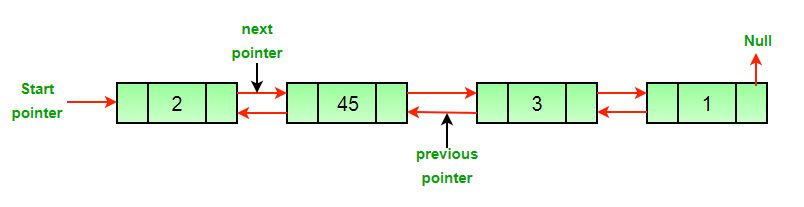
\includegraphics[scale = 0.7]{dll.jpg}
\vspace{2mm}
The advantages of having two pointers is evident: We can travel backwards from a node, instead of having to get to the node from all the way from the front. This makes some operations easy, and adding in a tail pointer makes this data structure very powerful.
\newpage
\subsection{\Large Stacks}
\hspace{4mm} A Stack is an \textbf{abstract} data type. It is similar to a "stack" of books, and the functions in this data type are similar to how a stack of books can be manipulated in real life.\par

\begin{center}
 \begin{tabular}{| m{9em} | m{15em} | m{4.5em} |} 
 \hline
 \textbf{Function} & \textbf{Functionality} \\ [0.5ex] 
 \hline
 push(node) & Adds the node to the front \\ 
 \hline
 top() & Returns the top node\\
 \hline
 pop() & Removes the last node\\
 \hline
 empty() & Return True if the stack is empty\\
 \hline
 \end{tabular}
\end{center}

Stacks are also reffered to as \textbf{Last-in-First-Out} or \textbf{LIFO Queues}. As they are abstract, they may be implemented as follows:

\subsubsection{\Large Implementing Stacks using Arrays}
\hspace{4mm} It can be seen quite easily how a stack can be implemented using an array. However, one major constraint in using arrays is that \textbf{the maximum size of the stack should be known.} This is because the size of an array cannot be modified once it has been allocated. (A work-around would be to use Dynamic Arrays, but more on that later.)\par
\vspace{4mm}
The pseudo-code for the above functions would be as follows:
\vspace{2mm}
\begin{lstlisting}[basicstyle = \Large, language = python]
    def Push(node new):
        if free == capacity : 
            return False;
        val[free] = new;
        free = free + 1;
        return True;
    
    def top():
        return val[free - 1];
        
    #Here, Val is the array storing the nodes
    #free is an integer showing where the next free  space is
    
    def pop():
        if empty():
            return False;
        val[free - 1] = None;
        free  = free - 1;
        return True;
    
    def empty():
        if val[0] == None:
            return True;
        else:
            return False;
        
\end{lstlisting}
    
\vspace{3mm}
We can clearly see from the above code that stacking fails if the capacity is exceeded. Also, notice that all the functions take $O(1)$ time to complete.

\subsubsection{\Large Implementing using Linked Lists}
\hspace{4mm} Linked lists have an advantage over arrays because the size is indefinite. However, keep in mind that we are using a singly-linked list with a tail pointer. If the tail pointer had not been present, the operations would've become $O(n)$.\par
\vspace{4mm}
Pseudo-code is as follows:

\begin{lstlisting}[language = python, basicstyle = \Large]
    def push(node new):
        #Changing pointer of last node
        ((tail -> last_node).next) = new;
        #changing the tail pointer
        tail = new;
    
    def top():
        return (head -> first_node);
    
    def pop():
        if empty():
            return False;
        else:
            head = head.next;
            return True;
    
    def empty():
        if head == Null;
            return True;
        else:
            return False;
    
\end{lstlisting}

\subsection{\Large Queue}
\hspace{4mm} This is similar to a real-life queue, in the fact that the people are put into a line and the first one in is the first one out; \textbf{FIFO Queue}. This is also an abstract data type. The functions in this are similar to that of a Stack, so we will not delve into much detail about the pseudo code here.\par

\begin{center}
 \begin{tabular}{| m{9em} | m{15em} | m{4.5em} |} 
 \hline
 \textbf{Function} & \textbf{Functionality} \\ [0.5ex] 
 \hline
 push(node) & Adds the node to the front \\ 
 \hline
 top() & Returns the top node\\
 \hline
 pop() & Removes the \textbf{FIRST} node\\
 \hline
 empty() & Return True if the stack is empty\\
 \hline
 \end{tabular}
\end{center}

\subsubsection{\Large Circular Queue in Arrays}
\hspace{4mm} The general pseudo code for the \texttt{pop()} in array would be:

\begin{lstlisting}[language = python, basicstyle= \Large]
    def Pop():
        result = val[0];
        i = 1
        while i < capacity:
            val[i-1] = val[i];
            i = i+1;
        return result;
\end{lstlisting}

However, this would take $O(n)$ order of time to be done. A faster way is to use a \textbf{HEAD} and a \textbf{TAIL} pointer to point where the queue starts and where the queue ends.\par

\begin{lstlisting}[basicstyle = \Large, language = python]
    def Pop():
        result = val[tail];
        Delete = val[tail];
        cycle(tail);
        return result;
        #Cycle() increases the value of tail by one   and if tail == capacity, it makes it's value 0 
\end{lstlisting}

This method makes the function to follow $O(1)$ time, and is thus faster.

\subsection{\Large Tree}
\hspace{4mm} As we all know, trees are used extensively in the representation of data. They consist of a node, and contain subsequent smaller branches which lead downwards. Formally in computer science, trees are recursively defined as follows:\par
\vspace{4mm}
\noindent \texttt{Tree is either empty \textbf{OR} points to nodes with smaller trees.}\par
\vspace{4mm}
\noindent Some terms are to be defined before we proceed further:
\begin{itemize}
    \item \textbf{Root:} The topmost node of the tree
    \item \textbf{Child: } Immediate node(s) below the current node
    \item \textbf{Ancestor: }All the modes above the current node
    \item \textbf{Descendants: }All the nodes below the current node
    \item \textbf{Sibling: }Nodes with the same parent
    \item \textbf{Leaf: }Nodes with no children
    \item \textbf{Level: }(Depth from the root) + 1
    \item \textbf{Height: }(Max distance from the leaves) + 1
    \item \textbf{Forest: }Collection of trees
\end{itemize}

A \textbf{Binary Tree} is a tree in which each node has a maximum of two sub-nodes. A binary tree is very simple, yet is VERY powerful.\newpage

\subsubsection{\Large Traversal through a Binary Tree}
\hspace{4mm}As the name suggests, traversal means travelling. This topic refers to how we may travel through the tree and obtain the data in the nodes for further usage. The two main types of traversal are:
\begin{enumerate}
    \item Depth First
    \item Breadth First
\end{enumerate}
\subsubsection*{\Large Depth First Traversal}
\hspace{4mm} This type of traversal has the program running through the binary tree through each of the consecutive branches. The pseudo-code for a function which prints elements traversing in this way would be:\par
\vspace{3mm}
\begin{lstlisting}[basicstyle = \Large, language = python]
    #Node is a class with the stored integer, pointers to the left and right side.
    
    def PrintTreeElem(node elem):
        if left is not NULL:
            PrintTreeElem(left);
        print stored;
        if right is not NULL:
            PrintTreeElem(right);
        
\end{lstlisting}
\vspace{4mm}
\hspace{4mm}Notice that we are printing the elements of Left node first, then the node itself, then the right node. This manner is called \textbf{InOrder}. If we print the node itself first, it is called \textbf{PreOrder}, and if we print it last, it is called \textbf{PostOrder}.

\subsubsection*{\Large Breadth First Traversal}
\hspace{4mm} This type of traversal implies that we are going to be printing out all the elements at the same level from the root node first, and we then start the process again with the nodes at the next level.
\newpage
The Pseudo-code for Depth First Traversal is as follows:
\vspace{2mm}
\begin{lstlisting}[basicstyle = \Large, language = python]
    def Breadth(node root):
        queue q;
        q.add(root)
        while q not empty:
            write q[0], q.pop()
            q.add(left), q.add(right)
            
\end{lstlisting}
\vspace{3mm}
\hspace{4mm} Also, understand that this works not only for a binary tree, but also for a general tree. The pseudo code for a general tree would be:
\vspace{3mm}
\begin{lstlisting}[language = python, basicstyle = \Large]
    def Breadth(node root):
        queue q;
        q.add(root)
        while q not empty:
            write q[0], q.pop()
            for subnode of q[0]:
                q.add(subnode)
\end{lstlisting}
\vspace{3mm}
This is how breadth first traversal works. We can use other forms of storage such as an array, or a linked list in place of a queue.

\subsection{\Large Dynamic Arrays}
\hspace{4mm} The arrays which we have discussed earlier are "static" in nature. That is, they cannot be modified with regards to their size. Once their size has been set, they become fixed. A logical way around this to make a "Dynamic" array.\par
\vspace{4mm}
These aren't necessarily abstract, and they are implemented in most languages. For example, Dynammic arrays in C++ are included in the \texttt{\#include <vector>} standard library, and in python we only have a Dynamic array.\par
\vspace{4mm}
The append function, in particular needs modification as we can see in the pseudo code below. The size of the array is doubled, and the elements are copied.

\begin{lstlisting}[language = python, basicstyle = \Large]
#Dynamic array for storing integers
    def append(int x):
        if head < capacity:
            val[head] = x
        else:
            n_val[2*capacity]
            n_val[0, 1.. (capacity - 1)] = val
            n_val[capacity] = x
            capacity = 2*capacity
            
\end{lstlisting}

\subsubsection{\Large Amortized Time Analysis}
\hspace{4mm} We can easily look at the code and say that the time taken for appending the new element is of $O(n)$ order. This is because all the elements have to be copied over to the new array. This seems wrong, as an array, by definition, must have \textbf{Constant Time access}.\par
\vspace{4mm}
Are we really right in thinking about the time to be $O(n)$ order? We can look at an \textbf{Amortized} analysis, or in more common terms, average analysis of the time.\par
\vspace{4mm}
\noindent Amortized Analysis tells us to take the average of the time taken for $n$ consecutive operations. For the appending function in the dynamic array, it shall be: $$\frac{\sum_{i=0}^{i=(n-1)}O(1) + O(n)}{n} = \frac{O(n)}{n} = O(1)$$
Therefore, we can see that although the max time taken for appending a new integer is $O(n)$, on average, dynamic arrays still have Constant Time Access.(They wouldn't be called arrays otherwise)
\newpage

\subsection{\Large Priority Queues}
\hspace{4mm} A priority queue is an abstract data type in which every element is assigned a \textbf{priority}, and the ones with the highest priority are extracted first. A real-life analogy to this would be how some airplane tickets have "classes", and the classes with the higher priority are allowed to board first. \par
\vspace{4mm}
The elements in a priority queue must be akin to elements in a bag. The elements need not necessarily be ordered inside the bag, but the following functions must be performable.\par


\begin{center}
 \begin{tabular}{| m{10em} | m{17em} |} 
 \hline
 \textbf{Function} & \textbf{Functionality} \\ [0.5ex] 
 \hline
 $insert(node, priority)$ & Inserts a node into the bag with the given priority \\ 
 \hline
 $extract()$ & Returns the node with highest priority\\
 \hline
 $pop()$ & Deletes the highest priority element\\
 \hline
 \end{tabular}
\end{center}
\vspace{4mm}
\hspace{4mm}The time taken for the functions is our indication of how good the data type has been implemented. We shall see some Naive Implementations and then a full fledged implementation of the Priority queues.

\subsubsection{\Large Naive Implementation - Arrays}
\hspace{4mm}We could easily use a dynamic array to store a priority queue. The first element of the dynamic array stores the element with the highest priority. \par
\vspace{4mm}
The pseudo-code for the above two functions would be as follows:
\begin{lstlisting}[language = python, basicstyle = \Large]
    def extract():
        return val[0]
    
    def insert(node, priority):
        for i from 0 to n:
            if (val[i].pri < priority):
                val[i, (i+1)..] = val[(i-1), i..]
                val[i-1] = node
                return
\end{lstlisting}

However, notice that the runtime for $insert(node, priority)$ is of the order of $O(n)$, because in the worst case scenario, all the elements would need to be moved forward. The next type of implementation would take care of this issue.

\subsubsection{\Large Implementation using Heaps}
\hspace{4mm} A heap is a binary tree in which the left and right sub-nodes of a node are smaller than or equal to the parent node. We can easily see that a heap could be used to represent a priority queue, with the root being the element with the highest priority.\par
\vspace{4mm}
\begin{center}
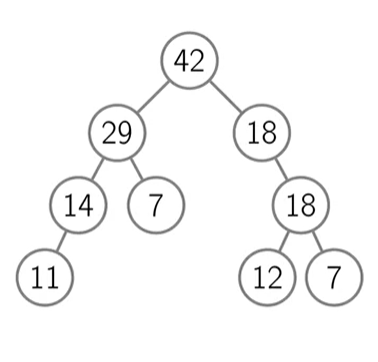
\includegraphics[]{tree.png}
\end{center}

Before we talk about the implementation of the above functions, let us first discuss the ways in which a wrong heap can be corrected. For example, in the above tree, if 11 and 42 were replaced with each other, we would need to have a method to correct the heap. $ShiftUp(node)$ and $ShiftDown(node)$ are the functions implemented for this purpose.\newpage

\begin{lstlisting}[language = python, basicstyle = \Large]
    def ShiftUp(node):
        if node.parent.pri < node.pri:
            swap node and node.parent
            ShiftUp(node.parent)
        else:
            return
    #ShiftDown will be implemented in the similar way
\end{lstlisting}
\vspace{3mm}
\hspace{4mm}Now that these both functions are defined, let's discuss how $pop()$ function would work. Well, instead of directly deleting the root and being left with two sub-trees, we swap the place of the root with any random leaf of the tree, and then employ $ShiftDown()$ for the new root. The pseudo-code for this would look like:
\vspace{3mm}
\begin{lstlisting}[language = python, basicstyle = \Large]
    def pop():
        temp = root
        while temp.left is not null:
            temp = temp.left
        #temp is now the left most leaf
        root = temp
        #replace root with temp
        ShiftDown(root)
        return
\end{lstlisting}
\vspace{4mm}
\hspace{4mm} This is much better than the dynamic array implementation because this takes $O(height)$ time to compute, compared to $O(n)$. However, this requires our tree to be somewhat branched out, because that would enable the tree to store the maximum number of nodes with the minimum height.\par
\vspace{3mm}
\theoremstyle{definition}
\begin{definition}{}
    A binary tree is said to be complete if all the levels of the tree are completely filled; except possibly the last one. The last level of the tree may be incomplete, but the present children must be filled from the left to the right.
\end{definition}
\newpage
Therefore, by modifying our codes appropriately to keep the binary tree complete, we can have the above functions run with the runtimes of $O(log_2^n)$, which is much better than the linear implementation that we had for the dynamic Arrays.

\subsection{\Large Hash Tables}
\theoremstyle{example}
\begin{example}
    You are the manager of a server, and you want to know the number of different IPs connecting to your server in the previous 60 minute interval, and also maintain a count of how many times the IP has connected.
\end{example}

This is a fairly common problem faced by servers, which we shall attempt to tackle now. IPs are generally given as $a.b.c.d$ where $0\leq a,b,c,d \leq 255$. For example, 101.23.40.120 is a valid IP. \par
\vspace{4mm}
Each number is less than 256, meaning each number can be stored in 8 Bits. This implies that the IP as a whole can be stored in 32 Bits. Let's try to tackle this problem using different data structures and see why the need for a new data structure has risen.

\subsubsection{\Large Implementing using Arrays}
\hspace{4mm}Because each IP takes up 32 Bits, all IPs can be stored in an array whose size is $2^{32}$. The mapping from the IP to the array address $(n)$ can be done as follows:
\[n = d + c\cdot 2^8 + b\cdot 2^{16} + a\cdot 2^{24}\]
All the values in the array will be initialized to $0$. Everytime an IP accesses the server, we would increase the value of the corresponding number in the array by one. This is good, as all the operations would take a $O(1)$, constant amount of time, which is what we need.\par
\vspace{4mm}
However, one BIG disadvantage of using this would be the memory it requires. We need to store a LARGE number of values without actually using most of them, because not all the IPs would connect to our server(obviously). This problem is worsened if we use IPv6, increasing the memory needed astronomically.

\subsubsection{\Large Implementing using Linked Lists}
\hspace{4mm} Because of the draw backs of arrays as show previously, we might be tempted to use Linked Lists. The nodes of the linked list would be storing the IP and the number of times that IP has connected to the server.\par
\vspace{4mm}
Pseudo-code which would be needed to run every time a new connection is detected would be:
\vspace{3mm}
\begin{lstlisting}[language = python, basicstyle = \Large]
    #Head refers to the head pointer
    def update(IP):
        temp = head
        while temp.next is not NULL:
            if temp.IP == IP:
                temp.count++
                return
            else:
                temp = temp.next
\end{lstlisting}
\vspace{3mm}
That is, we need to check through the ENTIRE linked list to see if the IP has been repeated already. This takes $O(n)$ time, and needs to be dome everytime. So although Linked lists saves us space, we lose the speed at which arrays were able to compute the values.

\subsubsection{\Large Best of both - Hash Tables}
\hspace{4mm} Simply speaking, Hash-Tables are arrays containing lists. We take all the IPs and we mathematically divide them into groups of approximately equal size. This is usually done by a function called the $Hashing-Function$.\par
\vspace{4mm}
The Hashing function takes the value of the IP and it returns the index of the array where it would be located in. Because the array index is obviously smaller than the total number of IPs, some IPs would return the same index when the Hashing-Function is passed. This is called as \textbf{Collision}.

\subsubsection{\Large Collision Handling}
\hspace{4mm} This refers to how Collisions are handled. In this case, if there is already a non-empty list at the array index, we scan this list. If the IP is already present in the list, it means that the IP has reconnected, so we can increase the count by one. If it isn't present we can append this IP with it's counter as one.\par
\vspace{4mm}
However, if the array element is empty, simply create a new empty list at that index and append this IP with it's counter as one. We can clearly see that this would be faster than only using arrays or lists.\par

\subsubsection{\Large Time Calculation and Increasing Speed}
\hspace{4mm} The time taken to look up whether an IP has connected would involve the following steps:
\begin{enumerate}
    \item Calculate the Array index from the Hashing Function - $O(1)$
    \item Look-up the array index - $O(1)$
    \item Scan through the list and check whether the IP is present - $O(length-of-list)$
\end{enumerate}
Therefore, the total time taken for looking up the IP would depend on the number of elements in the list. This is faster than arrays and list which would take $O(n)$ time. However, if our hashing function is bad, then all the IPs would be grouped into a sinle list which makes all the developments that we've done so far worthless.\par
\vspace{4mm}
Therefore, our Hashing function should distribute all the IPs uniformly so that the possibility for the is minimized. This involves multiple factors, and the definition of our Hashing Function determines how efficient our Data structure is, overall.

\newpage
\subsection{\Large Binary Search Trees}
\hspace{4mm} Suppose that we would like to be able to do a "Local" search for an element. That is, we would like to return all the elements withing a corresponding range; or the nearest neighbours of the given element. We also need to be able to insert new elements and remove already existing elements in the data structure.\par

\subsubsection{\Large Naive Implementation using Hash Tables}
\hspace{4mm} As we've discussed previously, Hash tables make inserting and deleting new elements fairly simple. However, the range search and finding the nearest elements would prove to be difficult as the elements which we are looking for need not be in the same part of the main array. \par
\vspace{4mm}
This would force us to search through the entire data structure and thus, would take a time of the order of $O(n)$. This is very much not ideal, and we thus look upon other data structures for this reason.

\subsubsection{\Large Implementation using Lists and Sorted Arrays}
\hspace{4mm} Sorted arrays work better in this case, as we can use \textbf{Binary Searching} for employing the Ranged Search and the Nearest Neighbours functions, as it takes only $O(log_2^n)$ order of time. However, it fails for inserting new elements because all the elements need to be shifted inorder for the array to remain sorted.\par
\vspace{4mm}
Linked Lists are immediately out of the picture, because we cannot aply a Binary search on them. This causes us to manually search the entire data structure, again taking $O(n)$ time.\par
\vspace{4mm}
However, these gripes feel similar to the ones we had when the need for trees had arisen. We shall therefore look at how a Binary tree is more efficient than all the data structures that we have studied so far.

\subsubsection{\Large Implementation of the Binary Search Tree}
\hspace{4mm} As the name suggests, a Binary Search Tree is a Binary tree with a special property that the left child of any node is smaller than the parent node and the right child of any node is greater than or equal to the parent node.\par
\vspace{4mm}
The pseudo-code for the above mentioned function, namely,\newline$RangedSearch()$, along with some other important functions is shown below.\par
\vspace{7mm}
\begin{lstlisting}[language = python, basicstyle = \Large]
    #next() gives the next biggest element stored
    def next(node N):
        if N.right is not NULL:
            temp = N.right
            while temp.left is not NULL:
                temp = temp.left
            return temp
        else:
            #return nothing if N is the largest
            if N.parent is NULL:
                return
            temp = N.parent
            next(temp)
    
    #Using next(), we can write RangeSearch()
    #val is a list storing the results
    def RangeSearch(node low, node high):
        if low is in tree:
            val.append(low)
        low = next(low)
        while low less than high:
            val.append(low)
            low = next(low)
        return val
\end{lstlisting}

\vspace{4mm}
\hspace{4mm} The best part of doing stuff in this way that the run time of our algorithm here is dependent only on the height of the tree, that is, if our tree is balanced, the runtime is $O(log_2^n)$. We can also quite easily see that the time taken for adding and deleting a node from this tree would also be dependent on the height of the tree, thus making it's runtime logarithmic as well.\par
\vspace{4mm}
Therefore, in order to have a good run-time, our trees need to be shallow. Do not confuse the properties mentioned after this with the properties discussed with heaps, as they are two completely different data types.

\subsubsection{\Large Balancing Trees - AVL Property}
\theoremstyle{definition}
\begin{definition}
    A Binary Tree is said to be AVL if the heights of both the children of any node(if the node has two children) differ atmost by 1.
\end{definition}
We can very clearly see that Binary trees which satisfy the AVL property are going to be shallow. Inorder for AVL property to be satisfied, we need to define some functions for us to be able to modify the Binary tree.\par
\vspace{4mm}
The functions which we would need to define would be $Rot\_L(node)$ and $Rot\_R(node)$, and their functionality would be as shown in the following figure:\par
\begin{center}
    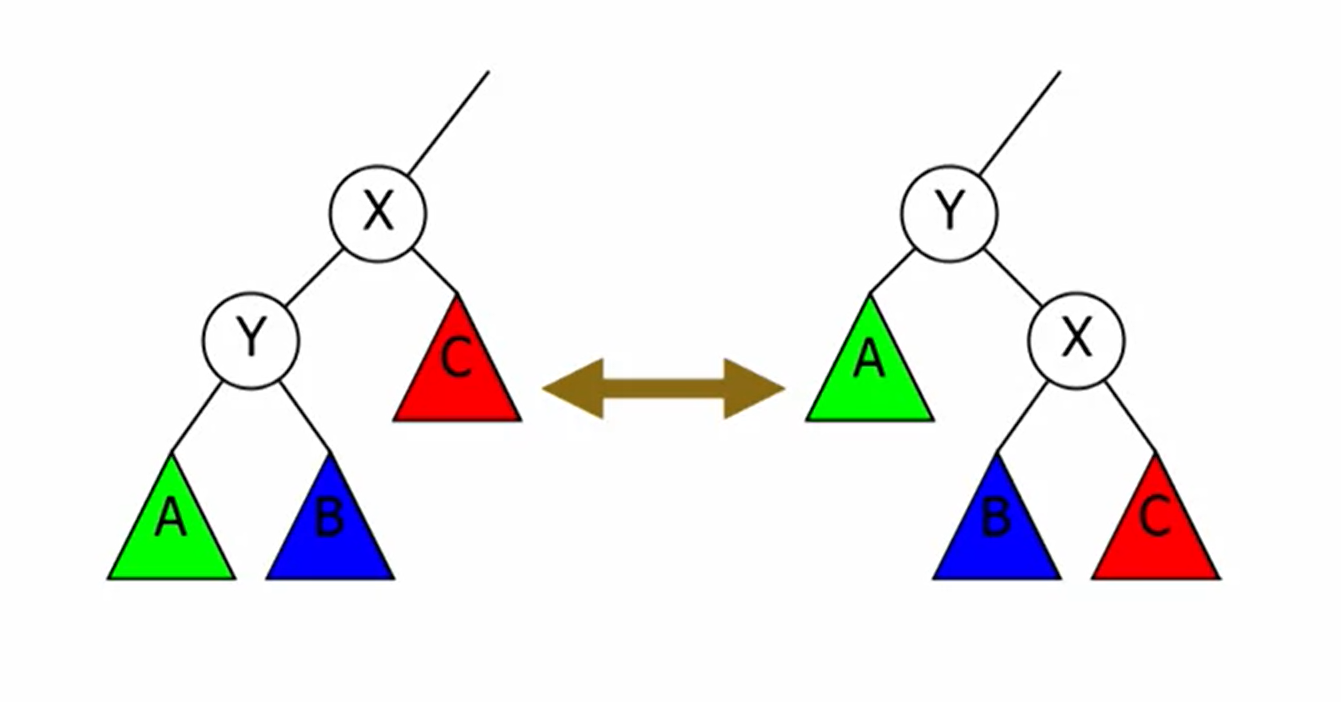
\includegraphics[scale = 0.6]{rot.png}
\end{center}
Implementing this feature is pretty simple, we need to check the tree after every insertion or deletion for the AVL Property. If the AVL property is not satisfied, we can use the rotate functions accordingle.\par
\vspace{4mm}
The heights need not be calculated on the go, but rather, they can be stored in the node itself. This would further speed up the process and make the entire tree faster. However, note that whenever any modification to the tree is done i terms of its structure, like, rotations, insertions and Deletions, all the values of height need to be recomputed. The pseudo-code for this would be as follows:
\vspace{3mm}
\begin{lstlisting}[language = python, basicstyle = \Large]
    #Note that Dynamic Programming can't be used
    #As nothing is repeated necessarily
    def Calc_Ht(node root):
        height = 1 + max(Calc_Ht(root.left), Calc_Ht(root.right))
        return height
\end{lstlisting}

\section{\Large Algorithms on Graphs}

\theoremstyle{definition}
\begin{definition}
    An Undirected Graph is a collection of vertices $(V)$, and Edges $(E)$ which connect pairs of Vertices.
\end{definition}

The above given definition is how graphs are defined formally. The vertices may be represented by points, and the edges may be represented by lines connecting the points. Some examples of Graphs in practical usage would be how social networks are represented and the such.\par
\vspace{4mm}
Edges generally connect two different Vertices but this need not always be the case. An edge which connects a vertex to itself is called as a \textbf{"Loop"}. Similarly, We can have multiple vertices between two vertices, but they are not considered generally.\par

\begin{center}
    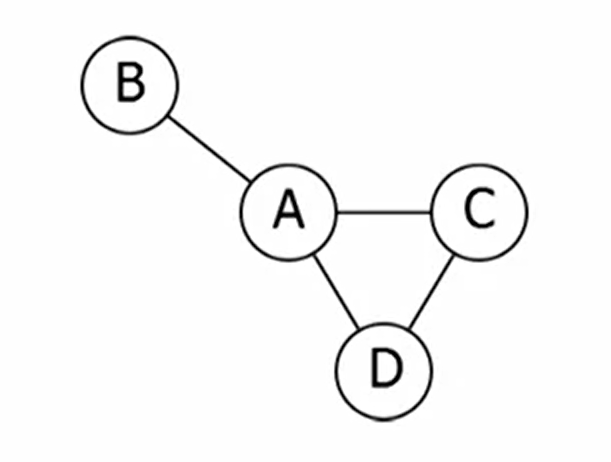
\includegraphics[scale = 0.8]{graph.png}
\end{center}

The above image is an example of a graph in which the vertices are A, B, C and D and the edges are the lines connecting the vertices. Notice that all the vertices need not be connected with each other; and there may be some vertices which are not connected to any vertices at all!\par

\subsection{\Large Representing Graphs}
\hspace{4mm} We have seen in the above image how graphs may be represented VISUALLY. However, they also need to be represented in such a manner that operating with them is easy, fast and efficient.
Some of the ways in which Graphs can be represented is as follows:

\begin{enumerate}
    \item Edge List
    \item Adjacent Matrix
    \item Adjacent List
\end{enumerate}

\textbf{Edge List} is pretty self-explanatory. All the edges are stored in a list, and when required, they can be looked up from the list.\par
\vspace{4mm}
\textbf{Adjacent Matrix} is an $|V|\times |V|$ matrix in which all elements are initialised to Zero. The cell $(1, 2)$ is marked as $1$ if there id an edge between Vertex 1 and Vertex 2. Notice that this array must be Symmetric.\par
\vspace{4mm}
\textbf{Adjacent List} is also pretty self explanatory. For every Vertex, we store a corresponding list as to which vertices are adjacent to it. Therefore, if we have $|V|$ vertices, we would have $|V|$ corresponding lists as well.
\vspace{6mm}
\begin{center}
 \begin{tabular}{| m{8em} | m{5em} | m{6em} | m{8em} |} 
 \hline
 \textbf{Storage Method} & \textbf{Edge?} & \textbf{List Edges} & \textbf{List Neighbours} \\ [0.5ex] 
 \hline
 Edge List & $\Theta (E)$ & $\Theta (E)$ & $\Theta (E)$ \\ 
 \hline
 Adjacent Matrix & $\Theta (1)$ & $\Theta (|V|^2)$ & $\Theta (|V|)$ \\
 \hline
 Adjacent List & $\Theta (deg)$ & $\Theta (E)$ & $\Theta (deg)$ \\
 \hline
 \end{tabular}
\end{center}

We will be looking at an Adjacent list From here on, as it's easy enough to implement and it is more efficient in the broader sense.\newpage

\subsection{\Large Computing Runtime}
\hspace{4mm} We've previously talked about how runtimes of an algorithm may be computed. We've been using the $Big-O$ Notation ever since, and it has worked quite well till now. However, ALL the runtimes that we've discussed till now only rely on ONE variable, the size of the input, which makes comparision easy. That's no longer the case here.\par
\vspace{4mm}
In graphs, the run time of the algorithm is going to depend on both $|V|$ and $|E|$. This makes it tough because we cannot really compare two algorithms whose runtimes are $O(|V|^{\frac{3}{2}})$ and $O(|E|)$. Thus, we define another classification of the graphs:

\begin{enumerate}
    \item \textbf{DENSE: } A graph is said to be Dense, if mostly all the vertices are interconnected with each other by a vertex. In a dense graph, $|E|\approx |V|^2$.
    \item \textbf{SPARSE: } A Graph is called Sparse, if the weaving isn't very complex. Here $|E|\approx |V|$.
\end{enumerate}
\vspace{9mm}
\begin{center}
    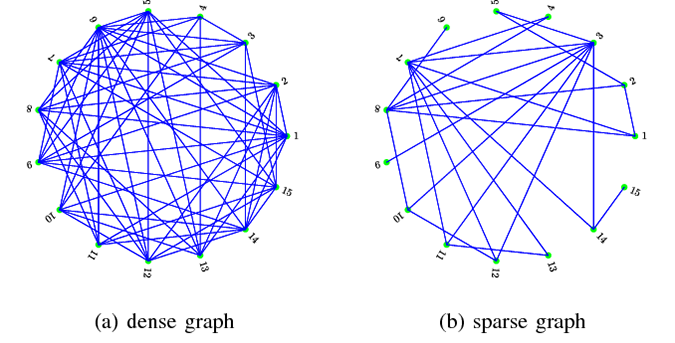
\includegraphics[scale = 0.6]{yeehaw.png}
\end{center}
\newpage

\subsection{\Large Graph Exploration}
\hspace{4mm} This is pretty self-explanatory. We shall aim to write an algorithm which can "explore" our graph and see how different vertices are connected to each other. It is intuitively the first step do be done as any other complex algorithm tat we'd write would surely use this as it's subpart.\par
\vspace{4mm}
Before we write an algorithm for this, let us formally define what a "path" is in an Algorithm.
\theoremstyle{definition}
\begin{definition}
    A Path is a collection of $n$ vertices like $\{v_1, v_2, .. v_n\}$ such that all $(v_i, v_{i+1})$ are connected by an edge.
\end{definition}
\vspace{3mm}
We shall first present the Pseudo-code for an algorithm which, when presented with a node, returns a list containing all the reachable nodes from the input node.\par
\vspace{3mm}
\begin{lstlisting}[language = python, basicstyle = \Large]
    #discover is the list storing the nodes
    #node has bool visit, which is made True once visited
    #neighbours of a node stored in list adjacent
    
    def reach(node s):
        s.visit = True
        discover.append(s)
        for temp in s.adjacent:
            if temp.visit is False:
                reach(temp)
        return discover
\end{lstlisting}

\vspace{4mm}
Now that $reach()$ has been properly defined, let us write the pseudo-code for a Depth-First Search Algorithm. This need not do much as of now, as it can be modified later to suit our needs. As of now though, this algorithm should be able to traverse and return all the vertices present in the given graph BY TRAVERSING THE GRAPH.
\newpage
\begin{lstlisting}[language = python, basicstyle = \Large]
    #nodes is the list which stores all nodes
    def DFS():
        create empty list called nodes
        for node in tree:
            if node.visit is False:
                nodes.append(reach(node))
\end{lstlisting}
\vspace{4mm}
Understand that the algorithm's run-time would be of the order $O(|V|+|E|)$. It's simple enough to be seen directly without any outright explanation. This is \textbf{Linear Time} in case of Graphs.

\subsubsection{\Large Connected Components}
\hspace{4mm} Connected Components are like "islands" when we look at a pictorial representation of graphs.
\theoremstyle{definition}
\begin{definition}
    A set of vertices $(S)$ is said to be a Connected Component if for every $u, v \in S$, There exists a path connecting $u$ and $v$.
\end{definition}

Notice that this relation is Equivalence in nature. We can modify our $DFS()$ algorithm to easily count the number of Connected Components in the given graph, and also find out which nodes belong to the same connected component. We first add a new variable called \texttt{cc} in the node to store the label of the connected component. The Pseudo-Code is:
\vspace{3mm}
\begin{lstlisting}[language = python, basicstyle = \Large]
    
    def DFS():
        #create label here
        num == 1
        create empty list called nodes
        for node in tree:
            if node.visit is False:
                nodes.append(reach(node, num))
                #increase label
                num = num + 1 
    
    
    
    def reach(node s, int num):
        s.visit = True
        s.cc = num #storing the label here
        discover.append(s)
        for temp in s.adjacent:
            if temp.visit is False:
                reach(temp)
        return discover
 
\end{lstlisting}
\vspace{4mm}
\hspace{4mm} Now, once the labels have been set, we could simply scan through the vertices and pick out the ones we need. This algorithm also takes $O(|V|+|E|)$ time as nothing has changed significantly, and only constant time operations have been added.

\subsection{\Large Directed Graphs}
\hspace{4mm} The graphs that we have discussed so for have no directional component for their edges. This means that the edge can be traversed from either end to the other. However, if an edge only allowed for travel in one direction, then the graph would be called a "Directed Graph".\par
\vspace{4mm}
If we think about it, Directed graphs are more useful in applications of road mapping and the such because not all roads would allow passenger to move in both the directions freely. Thus, defining these graphs is important and necessary.\par
\vspace{4mm}
We can simply modify the definition of Adjacent list to account for this. The vertices which are present in the adjacent list of a vertex $v$ all have a directed edge from $v$ to the corresponding vertex.\par

\begin{enumerate}
    \item \textbf{SINKS: }The vertices which only have edges pointing towards them.
    \item \textbf{SOURCES: }The vertices which only have edges pointing away from them.
\end{enumerate}

\subsubsection{\Large Linear Ordering}
\hspace{4mm} A Linear arrangement of the vertices in the given graph which satisfies the directional orders in the graphs is called as a Linear Ordering. The following image makes it more clear:
\vspace{4mm}
\begin{center}
    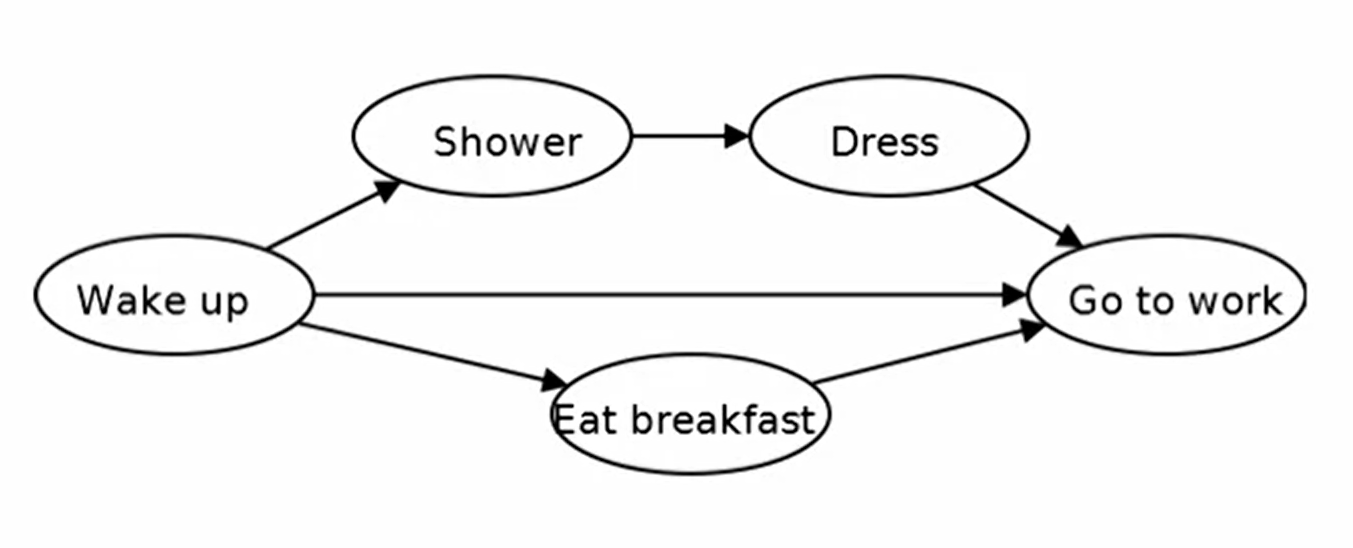
\includegraphics[scale = 0.56]{lo1.png}
    \newline
    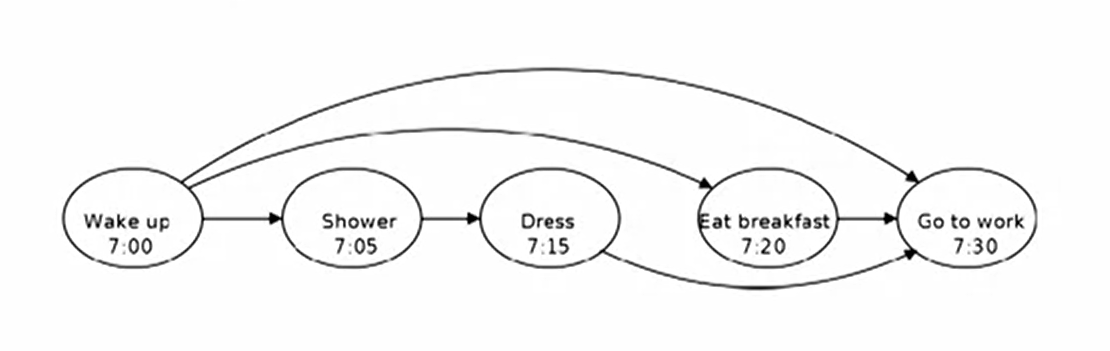
\includegraphics[scale = 0.7]{lo2.png}
\end{center}
\vspace{4mm}
 It can be clearly seen that Linear Ordering of a Directed Graph is possible \textbf{IFF} there are no cycles present in the graph. A directed Graph which has no cycles present in it is called as \textbf{Directed Acyclic Graph}.\par
 
 \subsubsection*{\Large Algorithm for Linear Ordering a graph}
\hspace{4mm} 
The logic behind this is pretty simple. We first find the a sink in the graph. (A DAG must have atleast one sink) We then append this graph to the last of the LO. We then remove this vertex from the graph and iterate till there are no more vertices left in the Graph.

\subsubsection*{\Large Strongly Connected Components}
\hspace{4mm} Simply put, this is similar to the Connected-Components that we described earlier for undirected graphs, but for Directed Graphs. 

\subsection{\Large Dijkstra's Algorithm}
\hspace{4mm} As we can realise, graphs can be used pretty easily to represent a map of an area with the edges representing nodes. The next logical step would be to develop an algorithm for finding the shortest path between two vertices. The problem statement has been stated properly below.

\theoremstyle{example}
\begin{example}
    Given a Graph and a starting vertex $S$. Each edge has a corresponding "weight", i.e., the time taken to traverse the edge. The weight is Non-Zero. Find the minimum time it would take to reach ANY vertex from the vertex $S$.
\end{example}

Dijkstra's Algorithm is a simple way of achieving this. We have a variable in each of the vertex which stores the minimum distance from $S$, let it be called $dist$.

\begin{enumerate}
    \item We first instantiate $dist$ in $S$ to be $0$, and then all the others are instantiated to $\infty$.
    \item The vertices which have their $dist$ figured out are stored in a set called $R$. Calculate the possible values of $dist$ for it's neighbours(which are not in $R$) by using $dist$ of the current vertex.
    \item  If the calculated value is smaller than what is stored, we replace the stored with the calculated value.
    \item Choose the vertex which is not in $R$, which has the lowest value of $dist$ to be the current vertex and iterate from step 2.
    \item When all belong to $R$, all the distances are known.
\end{enumerate}

We can go further and add another variable called $prev$ which points to the node from where we arrived at the current node. This can be useful if we are trying to obtain the path in which our algorithm travels. The pseudo-code would be:
\vspace{3mm}
\begin{lstlisting}[language=python, basicstyle = \Large]
# G is the Graph, S is the Source
def Dijkstra(G, S):
    S.dist = 0
    v = S
    #infinity refers to very large number
    rest all Vertices set dist = infinity
    create PriorityQueue(Q) and store all vertices
    while Q is not empty:
        for all w neighbours of v:
            if v.dist + E(v,w) < w.dist:
                w.dist = v.dist + E(v,w)
  #ExtractMax() returns and removes least priority
        v = ExtractMax(Q)
        
\end{lstlisting}
\vspace{4mm}
From this we can calculate the minimum distance from the mentioned source to any vertex in the entire graph. This algorithm forms the basis of another efficient algorithm called the $A^{*}-Algorithm$ which can be used to easily find the shortest distance between any two given vertices.

\subsection{\Large $A^*-Algorithm$}
\hspace{4mm} As discussed earlier, this algorithm is just a small variation of the Dijkstra's Algorithm that we've discussed earlier. This algorithm involves a \textbf{Directed Search}, meaning that the algorithm tends to prioritize the choices which take it closer to the target amongst all the choices.\par
\vspace{4mm}
\theoremstyle{definition}
\begin{definition}
    \textbf{Potential Function} is a function which maps all the vertices in the graph to a numerical value. It is denoted by $\pi(v)$.
\end{definition}

Now that a Potential function has been defined, then next logical step is to use this potential function to re-define the edge weights of our graph again. Keep in mind that we are talking about a directed graph here.\par
\vspace{4mm}
The redefined edge weight for an edge from a vertex $u$ to another vertex $v$ is given by:
\[l_{\pi}(u,v) = l(u,v) - \pi(u) + \pi(v)\]

This poses another constraint; by definition, all the new edge weights must also be non-negative. The Potential Functions which satisfy this condition are said to be \textbf{Feasible}.\par
\vspace{4mm}
Let $s$ be the Starting Vertex and $t$ be the target vertex. There exist many paths, and the $i^{th}$ path is denoted by $P_i$. Notice that after redefining all the edges, the Path Length shall be:
\[l_{\pi}(P_i) = l(P_i) - \pi(s) + \pi(t)\]
That is, the path lengths only change by a constant. We can therefore also conclude from this that the \textbf{Shortest path is the same after conversion}, because all the paths differ from the original by a constant. Sure, the length has changed, but the path is still the same.\par
\vspace{4mm}
Therefore, we can apply Dijkstra's Algorithm to this modified graph and still end up with the shortest path for the original graph. If we were required to calculate the minimum length between the two vertices, we can get that from the new graph as well, as it differs by a constant.
\newpage

\section{\Large String Algorithms}
\hspace{4mm} Algorithms on Strings have an immense importance in our daily lives. Search Engines use these algorithms to provide us with the results which are related to our search, after scanning through Terabytes of Webpages in an instant.\par
\vspace{4mm}
These algorithms can also be used in Bio-informatics, to check how similar the DNA of two species is, or where the DNA of a person with a genetic disease and a healthy person differ. This shall involve scanning through a large number of strings, and the methods to do o shall be discussed below.\par
\vspace{4mm}
The Human Genome project, consisted of DNA from humans to be extracted and broken up randomly by enzymes. The fragments are then analyzed to get the sequence of the Amino Acids making up that part. Then an algorithm is tasked with scanning all these pieces and figuring out where each piece should be located, much like a jigsaw puzzle, in which the pieces can be overlapping, are randomly generated, and the final solution is Millions of Amino Acids long. This is where these algorithms come into play.\par
\vspace{4mm}
We shall look at some ways of checking whether given strings are sub-strings of a larger string, in an efficient manner.

\subsection{\Large Pattern Matching Algorithms}

\theoremstyle{example}
\begin{example}
    Given a main string $S$, and $n$ other strings $p_n$, check which of the $p_n$ are substrings of $S$, and where they are located in the main string as well.
\end{example}

The easiest solution would be to simply check for the first letter of the main with the first letter of $p_1$. This is the simplest solution, and it DOES work, but its VERY slow. The pseudo-code for the naive algorithm would be as follows:
\newpage
\begin{lstlisting}[language = python, basicstyle = \Large]
    #P[n] is the array with all the strings to be checked
    #S[0] refers to first letter of string
    #result is the array with the substrings
    def Naive_Matching(S, P[n]):
        result = []
        for i in range(n):
            j = 0
            while True:
                if S[j] !== P[i][j]:
                    break
                if j == len(P[i]):
                    result.append(P[i])
                j = j + 1
        return result

\end{lstlisting}
\vspace{4mm}
\hspace{4mm}Let's look at how this algorithm performs time-wise. It can be clearly seen that the time would be of the order $O(len(S)\cdot n)$, and in the case of the human genome, this would never get done for obvious reasons. \par
\vspace{4mm}
One reason why this algorithm is so slow is that we are needed to scan through the same string multiple times. We can modify the approach to be so that we are required to scan the string only once. The following method talks about this approach.

\subsubsection{\Large Trie-Matching the Smaller Strings}
\hspace{4mm} A "Trie" is a way of grouping together all the smaller strings efficiently and simply. A Trie is basically a Tree which stores the strings with the common alphabets acting as nodes. For example, the below structure is how the following sub-strings are stored:\par
\vspace{2mm}
\begin{center}
     ananas,
     and,
     antenna,
     banana,
     bandana,
     nab,
     nana,
     pan
\end{center}
\vspace{4mm}
\begin{center}
    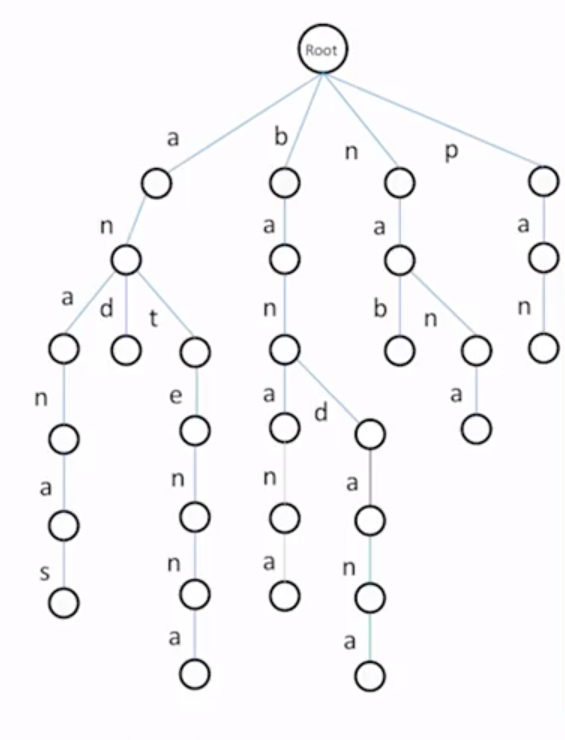
\includegraphics[scale = 0.5]{Trie_ss.png}    
\end{center}
\vspace{4mm}
\hspace{4mm} It can be seen clearly that this method would save a lot of time as we would be checking all the sub-strings at once, and this would obviously more faster. But would this be enough? Actually no, because we would still have the run-time would be $O(len(S)\cdot max(P[i]))$.\par
\vspace{4mm}
The time for this still be very high, and thus we are required to think of more efficient methods.
\newpage
\subsubsection{\Large More Efficient Trie-Matching}
\hspace{4mm} 
Instead of putting all the strings to be searched in a Trie, lets instead put the ORIGINAL STRING, i.e., $S$, in a Trie. In the above example, suppose $S =$ "PANAMABANANAS".\par
\vspace{4mm}
We then put all the possible sub-strings of $S$ into a Trie, as shown below. The sub-strings of $S$ would be "PANAMABANANAS", "ANAMABANANAS", and so on. The Leaves of the Trie are denoted by \$ sign, and it also stores the number where the Substring is located. This allows us to pin-point where the particular substring is present in the original string. \par

\vspace{3mm}
\begin{center}
    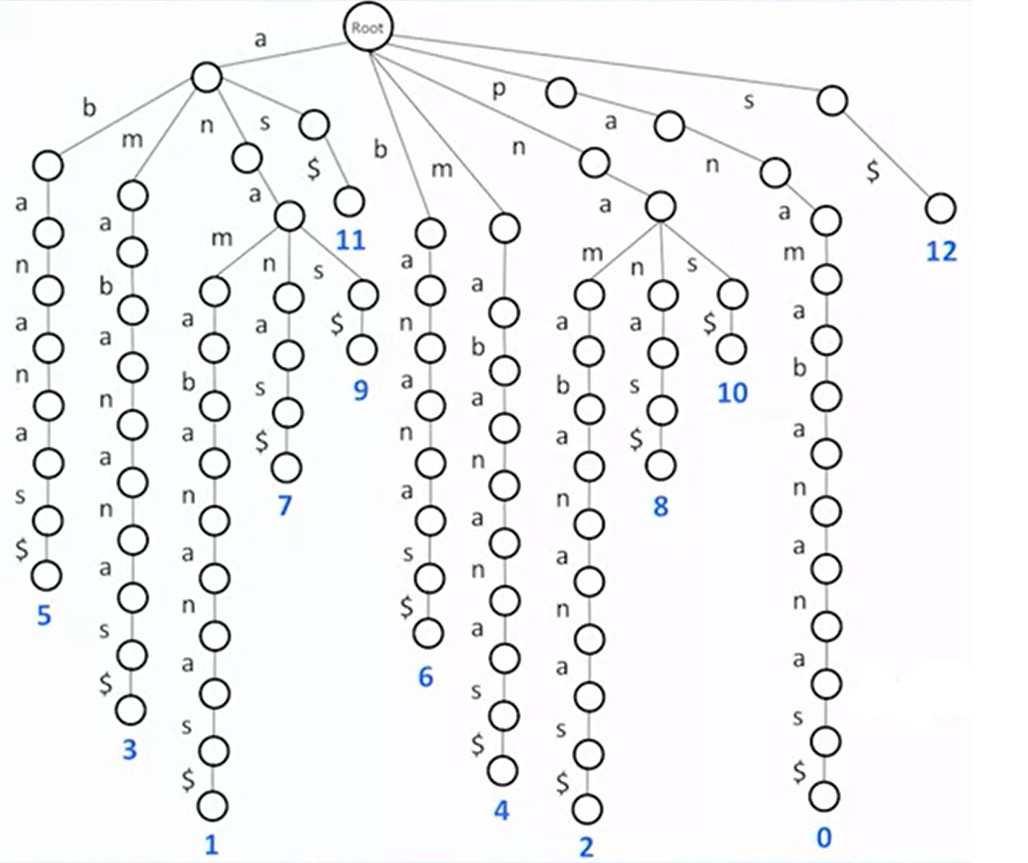
\includegraphics[scale = 0.75]{Final_Trie.jpg}
\end{center}
\vspace{3mm}
\newpage
Although this would make matching VERY fast, the space needed to store the sub-string is HUGE. By some quick math, we can see that the space needed to store a string of size $n$ would be $O(n^2)$; which is completely impractical.\par
\vspace{4mm}
We overcome this problem pretty simply. First, storing each letter of the word "BANANAS" in the left-most branch in a different node is a huge waste of space. We can simply store the entire word "BANANAS\$" in one leaf itself. Doing this to the above tree gives us this:\par
\vspace{2mm}
\begin{center}
    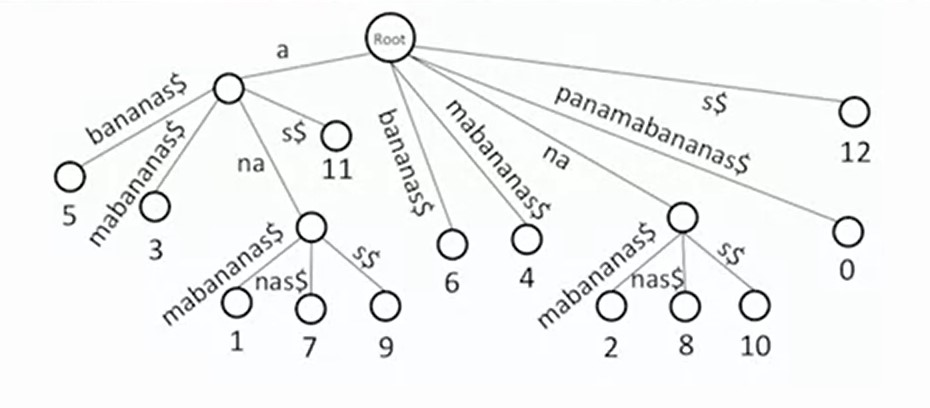
\includegraphics[scale = 0.77]{comp.jpg}
\end{center}
\vspace{3mm}
This STILL doesn't solve our problem, as we still need to store the entire sub-strings. However, we can work around this, pretty easily. Because a string can be accessed in constant-time, we can simply store the starting index and the length of the string. This DRASTICALLY reduces the space needed to store the string. The modified Trie is as follows:\par
\vspace{3mm}
\begin{center}
    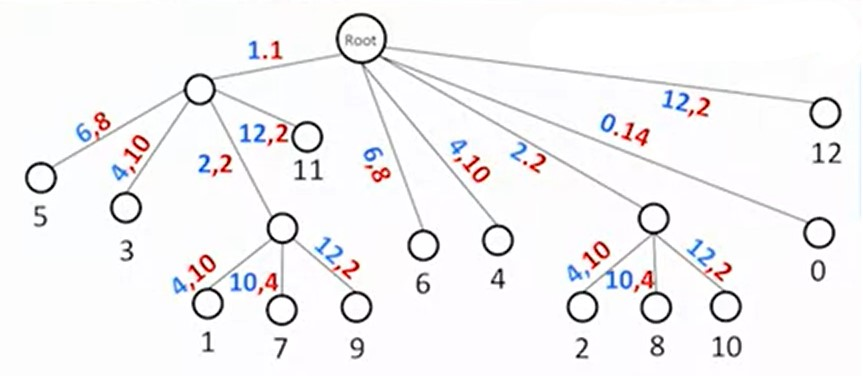
\includegraphics[scale = 0.5]{final.jpg}
\end{center}

\section{\Large References}
\begin{itemize}
    \item Coursera's Specialization Course
    \item Coursera's Data Structures and Algorithms Course
    \item Coursera's Courses on Graphs and Strings
    \item Tutorials by TutorialsPoint
\end{itemize}



\end{document}